\onehalfspacing
\section{Đề số 7}
\graphicspath{{./img/}}
\begin{bt} 
	\hfill
	\begin{enumerate}[1.]
		\item Tính $M=\left(\frac{0,4-\frac{2}{9}+\frac{2}{11}}{1,4-\frac{7}{9}+\frac{7}{11}}-\frac{\frac{1}{3}-0,25+\frac{1}{5}}{1 \frac{1}{6}-0,875+0,7}\right): \frac{2012}{2013}$
		\item Tìm $x$, biết: $\left|x^2+\right| x-1||=x^2+2$.
	\end{enumerate}
	\loigiai{
		\begin{enumerate}
			\item Ta có:\\[5px]
			$
			M=\left(\frac{0,4-\frac{2}{9}+\frac{2}{11}}{1,4-\frac{7}{9}+\frac{7}{11}}-\frac{\frac{1}{3}-0,25+\frac{1}{5}}{1 \frac{1}{6}-0,875+0,7}\right): \frac{2012}{2013}\\[5px]
			=\left(\frac{\frac{2}{5}-\frac{2}{9}+\frac{2}{11}}{\frac{7}{5}-\frac{7}{9}+\frac{7}{11}}-\frac{\frac{1}{3}-\frac{1}{4}+\frac{1}{5}}{\frac{7}{6}-\frac{7}{8}+\frac{7}{10}}\right): \frac{2012}{2013}\\[5px]
			=\left(\frac{2\left(\frac{1}{5}-\frac{1}{9}+\frac{1}{11}\right)}{7\left(\frac{1}{5}-\frac{1}{9}+\frac{1}{11}\right)}-\frac{\left(\frac{1}{3}-\frac{1}{4}+\frac{1}{5}\right)}{\frac{7}{2}\left(\frac{1}{3}-\frac{1}{4}+\frac{1}{5}\right)}\right): \frac{2012}{2013}\\[5px] 
			=\left(\frac{2}{7}-\frac{2}{7}\right): \frac{2012}{2013}=0\\[5px]
 			$
			KL: .....
			\item  Vì  $x^2+|x-1|>0 \text { nên }(1)=>x^2+|x-1|=x^2+2 \text { hay }|x-1|=2$
			\begin{enumerate}[+]
				\item Nếu $x \geq 1$ thì $\left({ }^*\right)=>x-1=2 \Rightarrow x=3$
				\item Nếu $x<1$ thì $\left(^*\right)=>x-1=-2 \Rightarrow x=-1$
			\end{enumerate}
			KL: .....
		\end{enumerate}
	} 
\end{bt}

\begin{bt}
	\hfill
	\begin{enumerate}[1.]
		\item Cho $a, b, c$ là ba số thực khác 0 , thoả mãn điều kiện:
		$$
		\frac{a+b-c}{c}=\frac{b+c-a}{a}=\frac{c+a-b}{b} \text {. }
		$$
		Hãy tính giá trị của biểu thức $B=\left(1+\frac{b}{a}\right)\left(1+\frac{a}{c}\right)\left(1+\frac{c}{b}\right)$.
		\item Ba lớp 7A, 7B, 7C cùng mua một số gói tăm từ thiện, lúc đầu số gói tăm dự định chia cho ba lớp tỉ lệ với 5:6:7 nhưng sau đó chia theo tỉ lệ 4:5:6 nên có một lớp nhận nhiều hơn dự định 4 gói. Tính tổng số gói tăm mà ba lớp đã mua.
	\end{enumerate}
	\loigiai{
		\begin{enumerate}
			\item \begin{enumerate}[+]
				\item Nếu $a+b+c \neq 0$\\[5px]
				Theo tính chất dãy tỉ số bằng nhau, ta có:\\[5px]
				$
				\frac{\mathrm{a}+\mathrm{b}-\mathrm{c}}{\mathrm{c}}=\frac{\mathrm{b}+\mathrm{c}-\mathrm{a}}{\mathrm{a}}=\frac{\mathrm{c}+\mathrm{a}-\mathrm{b}}{\mathrm{b}}=\frac{\mathrm{a}+\mathrm{b}-\mathrm{c}+\mathrm{b}+\mathrm{c}-\mathrm{a}+\mathrm{c}+\mathrm{a}-\mathrm{b}}{\mathrm{a}+\mathrm{b}+\mathrm{c}}=1 \\[5px]
				\text { mà } \frac{a+b-c}{c}+1=\frac{b+c-a}{a}+1=\frac{c+a-b}{b}+1=2 \\[5px]
				\Rightarrow \frac{a+b}{c}=\frac{b+c}{a}=\frac{c+a}{b}=2 \\[5px]
				\text { Vậy B }=\left(1+\frac{b}{a}\right)\left(1+\frac{a}{c}\right)\left(1+\frac{c}{b}\right)=\left(\frac{b+a}{a}\right)\left(\frac{c+a}{c}\right)\left(\frac{b+c}{b}\right)=8$ 
				\item Nếu $\mathrm{a}+\mathrm{b}+\mathrm{c}=0 \text { thì } \mathrm{a}+\mathrm{b}=-\mathrm{c}, \mathrm{b}+\mathrm{c}=-\mathrm{a}, \mathrm{c}+\mathrm{a}=-\mathrm{b}.\\[5px]
				\text { Vậy } B=\left(1+\frac{b}{a}\right)\left(1+\frac{a}{c}\right)\left(1+\frac{c}{b}\right)=\left(\frac{b+a}{a}\right)\left(\frac{c+a}{c}\right)\left(\frac{b+c}{b}\right)=\frac{-c}{a} \cdot \frac{-b}{c} \cdot \frac{-a}{b}=-1
				$
			\end{enumerate}
			\item Gọi tổng số gói tăm 3 lớp cùng mua là $x$ ( $x$ là số tự nhiên khác 0 )\\[5px]
			Số gói tăm dự định chia chia cho 3 lớp 7A, 7B, 7C lúc đầu lần lượt là: $a, b, c$\\[5px]
			Ta có: $\frac{a}{5}=\frac{b}{6}=\frac{c}{7}=\frac{a+b+c}{18}=\frac{x}{18} \Rightarrow a=\frac{5 x}{18} ; b=\frac{6 x}{18}=\frac{x}{3} ; c=\frac{7 x}{18}$ (1)\\[5px]
			Số gói tăm sau đó chia cho 3 lớp lần lượt là a', $\mathrm{b}^{\prime}, \mathrm{c}^{\prime}$, ta có:
			$$
			\frac{a^{\prime}}{4}=\frac{b^{\prime}}{5}=\frac{c^{\prime}}{6}=\frac{a^{\prime}+b^{\prime}+c^{\prime}}{15}=\frac{x}{15} \Rightarrow a^{\prime}=\frac{4 x}{15} ; b^{\prime}=\frac{5 x}{15}=\frac{x}{3} ; c^{\prime}=\frac{6 x}{15} (2)
			$$
			So sánh (1) và (2) ta có: $\mathrm{a}>\mathrm{a}^{\prime} ; \mathrm{b}=\mathrm{b}^{\prime} ; \mathrm{c}<\mathrm{c}^{\prime}$ nên lớp 7C nhận nhiều hơn lúc đầu\\[5px]
			 Vậy: $\mathrm{c}^{\prime}-\mathrm{c}=4$ hay $\frac{6 x}{15}-\frac{7 x}{18}=4 \Rightarrow \frac{x}{90}=4 \Rightarrow x=360$\\[5px]
			Vậy số gói tăm 3 lớp đã mua là 360 gói.
		\end{enumerate}
	} 
\end{bt}

\begin{bt}
	\hfill
	\begin{enumerate}[1.]
		\item Tìm giá trị nhỏ nhất của biểu thức $\mathrm{A}=|2 x-2|+|2 x-2013|$ với $x$ là số nguyên.
		\item Tìm nghiệm nguyên dương của phương trình $x+y+z=x y z$.
	\end{enumerate}
	\loigiai{
		\begin{enumerate}
			\item Ta có: \\[5px]
			$ A=|2 x-2|+|2 x-2013|=|2 x-2|+|2013-2 x| 
			\geq|2 x-2+2013-2 x|=2011$\\[5px] 
			Dấu "=" xảy ra khi $(2 x-2)(2013-2 x) \geq 0\\[5px] \Leftrightarrow 1 \leq x \leq \frac{2013}{2}$\\[5px]
            Do đó giá trị nhỏ nhất của A là 2011 khi $1 \leq x \leq \frac{2013}{2}$\\[5px]
			\item Vì $x, y, z$ nguyên dương nên ta giả sử $1 \leq x \leq y \leq z$\\[5px]
			Theo bài ra $1=\frac{1}{y z}+\frac{1}{y x}+\frac{1}{z x} \leq \frac{1}{x^2}+\frac{1}{x^2}+\frac{1}{x^2}=\frac{3}{x^2} \Rightarrow x^2 \leq 3 \Leftrightarrow x=1$\\[5px]
			Thay vào đầu bài ta có $1+y+z=y z \Rightarrow \mathrm{y}-\mathrm{yz}+1+\mathrm{z}=0$
			$$
			\begin{aligned}
			& \Rightarrow \mathrm{y}(1-\mathrm{z})-(1-\mathrm{z})+2=0 \\[5px]
			& \Rightarrow (\mathrm{y}-1)(\mathrm{z}-1)=2
			\end{aligned}
			$$
			TH1: $\mathrm{y}-1=1 \Rightarrow \mathrm{y}=2$ và $\mathrm{z}-1=2 \Rightarrow \mathrm{z}=3$\\[5px]
			TH2: $y-1=2 \Rightarrow y=3$ và $z-1=1 \Rightarrow z=2$\\[5px]
			Vậy có hai cặp nghiệm nguyên thỏa mãn $(1,2,3) ;(1,3,2)$
		\end{enumerate}
	} 
\end{bt}

\begin{bt}
	Cho $x A y=60^{\circ}$ có tia phân giác $\mathrm{Az}$. Từ điểm $\mathrm{B}$ trên $\mathrm{Ax}$ kẻ $\mathrm{BH}$ vuông góc với $\mathrm{Ay}$ tại $\mathrm{H}$, kẻ $\mathrm{BK}$ vuông góc với $\mathrm{Az}$ và $\mathrm{Bt}$ song song với $\mathrm{Ay}, \mathrm{Bt}$ cắt $\mathrm{Az}$ tại $\mathrm{C}$. Từ $\mathrm{C}$ kẻ $\mathrm{CM}$ vuông góc với Ay tại $M$. Chứng minh :
	\begin{enumerate}[a.]
		\item K là trung điểm của $A C$.
		\item $\triangle \mathrm{KMC}$ là tam giác đều.
		\item Cho $B K=2 \mathrm{~cm}$. Tính các cạnh $\triangle \mathrm{AKM}$.
	\end{enumerate}
	\loigiai{
		$$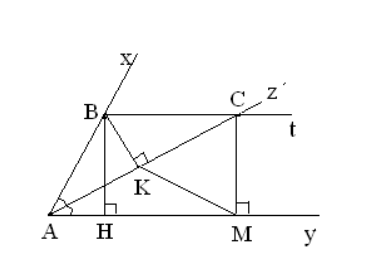
\includegraphics[width=0.45\textwidth]{7-4-lg.png}$$
		\begin{enumerate}
			\item $\triangle \mathrm{ABC}$ cân tại $\mathrm{B}$ do $C A B=A C B(=M A C)$ và $\mathrm{BK}$ là đường cao $\Rightarrow \mathrm{BK}$ là đường trung tuyến
			$\Rightarrow \mathrm{K}$ là trung điểm của $\mathrm{AC}$
			\item $\Delta \mathrm{ABH}=\Delta \mathrm{BAK}($ cạnh huyền + góc nhọn $)$\\[5px]
			$\Rightarrow \mathrm{BH}=\mathrm{AK}($ hai cạnh t.ư $)$ mà $\mathrm{AK}=\frac{1}{2} \mathrm{AC}$\\[5px]
			$\Rightarrow \mathrm{BH}=\frac{1}{2} \mathrm{AC}$\\[5px]
			Ta có : $\mathrm{BH}=\mathrm{CM}(\mathrm{t} / \mathrm{c}$ cặp đoạn chắn $)$ mà $\mathrm{CK}=\mathrm{BH}=\frac{1}{2} \mathrm{AC} \Rightarrow \mathrm{CM}=\mathrm{CK}\\[5px] \Rightarrow \Delta \mathrm{MKC}$ là tam giác cân (1)\\[5px]
			Mặt khác: $M C B=90^{\circ}$ và $A C B=30^{\circ}$
			$
			\Rightarrow M C K=60^{\circ}(2)
			$\\[5px] Từ (1) và (2) $\Rightarrow \Delta \Delta \mathrm{MKC}$ là tam giác đều
			\item Vì $\Delta \mathrm{ABK}$ vuông tại $\mathrm{K}$ mà góc $\mathrm{KAB}=30^{\circ} \Rightarrow \mathrm{AB}=2 \mathrm{BK}=2.2=4 \mathrm{~cm}$\\[5px]
			Vì $\triangle \mathrm{ABK}$ vuông tại $\mathrm{K}$ nên theo Pitago ta có:
			$$
			\mathrm{AK}=\sqrt{A B^2-B K^2}=\sqrt{16-4}=\sqrt{12}
			$$
			Mà $\mathrm{KC}=\frac{1}{2} \mathrm{AC} \Rightarrow \mathrm{KC}=\mathrm{AK}=\sqrt{12}$\\[5px]
			$\Delta \mathrm{KCM}$ đều $\Rightarrow \mathrm{KC}=\mathrm{KM}=\sqrt{12}$\\[5px]
			Theo phần b:\\[5px] $\mathrm{AB}=\mathrm{BC}=4$\\[5px]
			$\mathrm{AH}=\mathrm{BK}=2$\\[5px]
			$\mathrm{HM}=\mathrm{BC}$ ( $\mathrm{HBCM}$ là hình chữ nhật $)$\\[5px]
			$\Rightarrow \mathrm{AM}=\mathrm{AH}+\mathrm{HM}=6$
			
		\end{enumerate}
	}
\end{bt}

\begin{bt}
	Cho ba số dương $0 \leq \mathrm{a} \leq \mathrm{b} \leq \mathrm{c} \leq 1$ chứng minh rằng: $\frac{a}{b c+1}+\frac{b}{a c+1}+\frac{c}{a b+1} \leq 2$
	\loigiai{
		Vì $0 \leq a \leq b \leq c \leq 1$ nên:\\[5px]
$(a-1)(b-1) \geq 0 \Leftrightarrow a b+1 \geq a+b \Leftrightarrow \frac{1}{a b+1} \leq \frac{1}{a+b} \Leftrightarrow \frac{c}{a b+1} \leq \frac{c}{a+b}$ (1)\\[5px]
Tương tự: $\frac{a}{b c+1} \leq \frac{a}{b+c}$
(2) ; $\frac{b}{a c+1} \leq \frac{b}{a+c}$ (3)\\[5px]
Do đó: $\frac{a}{b c+1}+\frac{b}{a c+1}+\frac{c}{a b+1} \leq \frac{a}{b+c}+\frac{b}{a+c}+\frac{c}{a+b}$
(4)\\[5px]
Mà $\frac{a}{b+c}+\frac{b}{a+c}+\frac{c}{a+b} \leq \frac{2 a}{a+b+c}+\frac{2 b}{a+b+c}+\frac{2 c}{a+b+c}=\frac{2(a+b+c)}{a+b+c}=2$ (5)\\[5px]
Từ (4) và (5) suy ra: $\frac{a}{b c+1}+\frac{b}{a c+1}+\frac{c}{a b+1} \leq 2 \quad$ (đpcm)
	}
\end{bt}